\section{Problem Statement}

The increasing penetration of residential photovoltaic (PV) systems and behind-the-meter energy storage has introduced new operational challenges for microgrid energy management. While Battery Energy Storage Systems (BESS) offer significant potential for mitigating renewable intermittency and reducing electricity costs, their effective real-time control remains a challenging problem due to the stochastic and time-varying nature of both solar generation and household load demand.

A central challenge addressed in this thesis is the so-called \emph{optimizer’s dilemma} under uncertainty: how to approximate the performance of an offline optimal controller, one that assumes perfect foresight of future generation, load, and electricity prices, using only information available at the current time step.

High penetration of solar generation gives rise to the well-known \emph{duck curve} phenomenon~\cite{ref_duck_curve}, characterized by low net demand during midday hours and steep demand ramps in the evening. This temporal mismatch between energy production and consumption highlights the need for effective energy shifting strategies, where excess solar energy is stored during periods of high generation and discharged during peak demand periods. However, existing control approaches face several important limitations.

\begin{figure}[h]
    \centering
    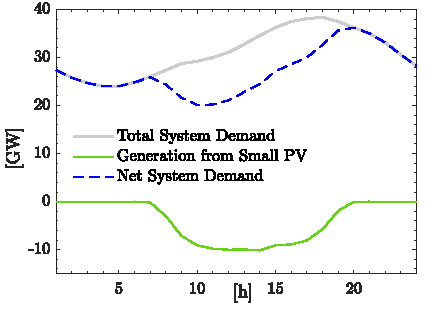
\includegraphics[width=0.8\textwidth]{Pages/fig/duck_curve.pdf}
    \caption{Illustration of the "Duck Curve" phenomenon, showing the impact of high solar penetration on net demand.}
    \label{fig:duck_curve}
\end{figure}

\begin{figure}[h]
    \centering
    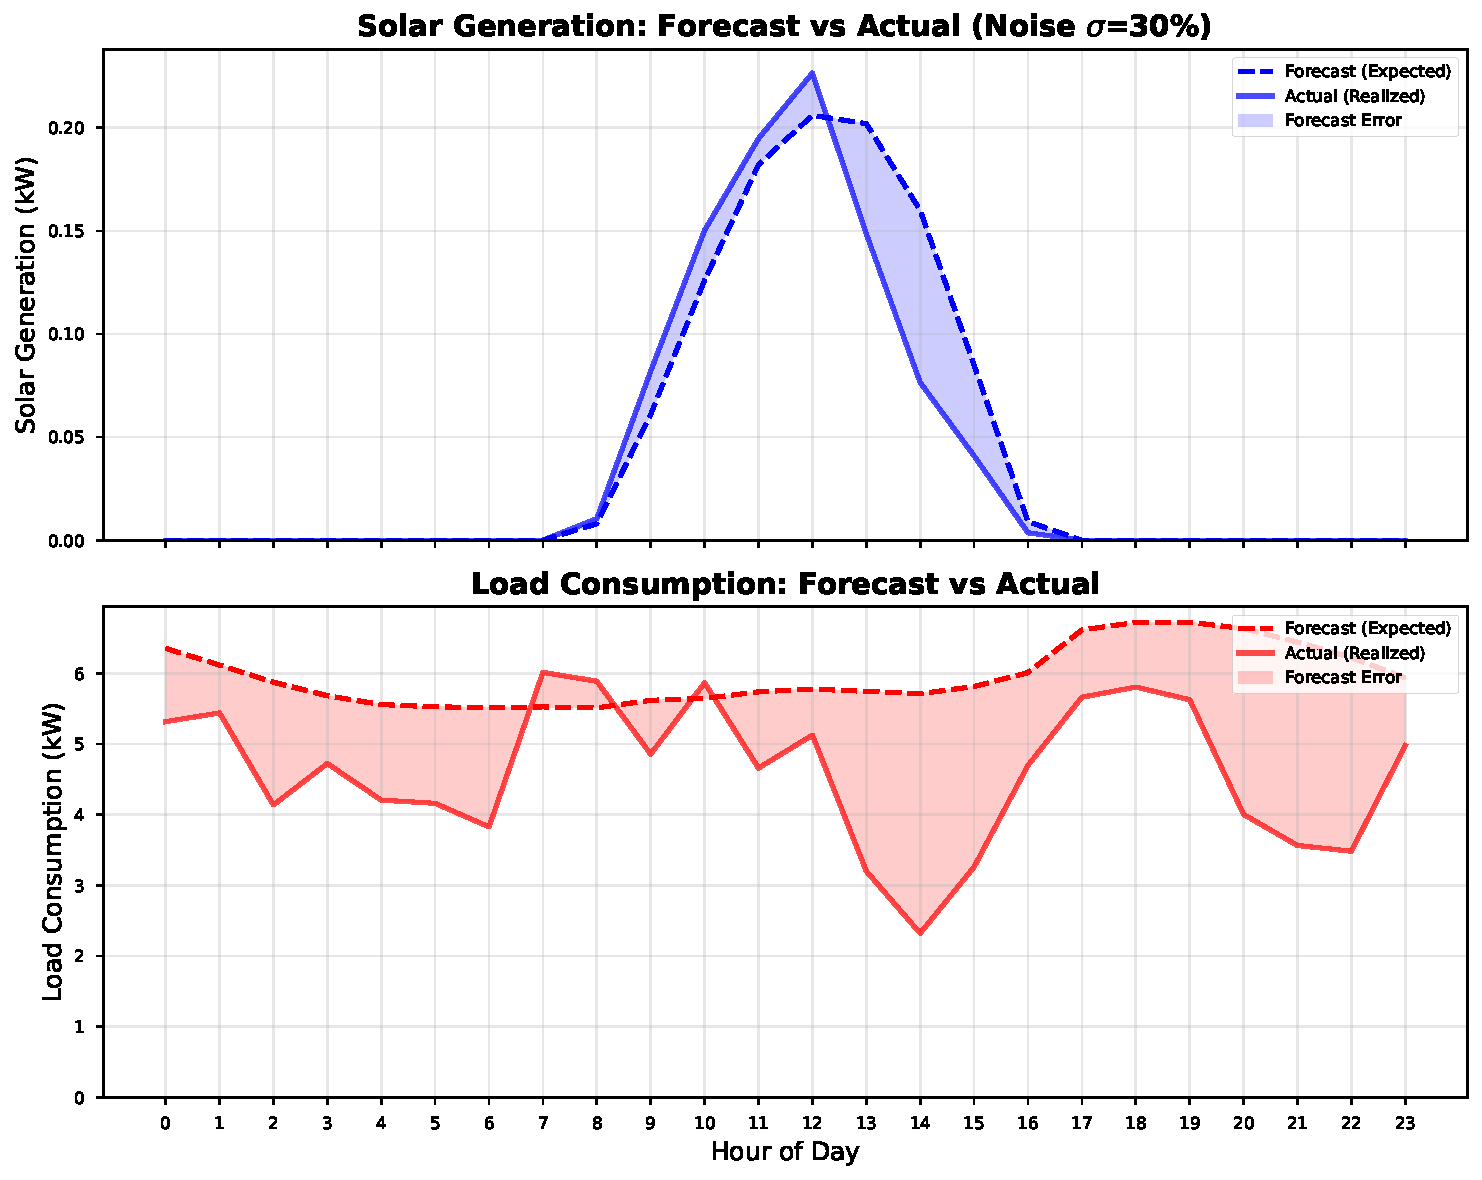
\includegraphics[width=1\textwidth]{Pages/fig/forecast_vs_actual.pdf}
    \caption{}
    \label{fig:forecast_error_illustration}
\end{figure}


Deterministic optimization-based methods, such as Linear Programming (LP) and Mixed-Integer Linear Programming (MILP), depend heavily on accurate forecasts of future solar irradiance and load demand. As illustrated in Figure~\ref{fig:forecast_error_illustration}, even relatively small forecast errors can cause substantial deviations from the optimal charging and discharging schedule. For example, an overly optimistic solar forecast may lead to premature battery discharge, resulting in insufficient stored energy and increased grid imports during high-price periods.

In addition, realistic battery modeling introduces significant computational complexity. While linear battery models are attractive due to their simplicity, they fail to capture non-linear characteristics such as variable charging efficiency and degradation effects. Incorporating these non-linearities into conventional optimization frameworks often requires simplifications that increase computational burden or reduce model fidelity~\cite{Xu2016}, limiting their suitability for real-time residential applications.

Heuristic and rule-based controllers offer computational efficiency and robustness but lack adaptability. These methods rely on fixed thresholds and predefined logic, which cannot dynamically respond to changing electricity prices, evolving load patterns, or unexpected weather conditions. As a result, they often fail to exploit inter-temporal arbitrage opportunities, leading to consistently suboptimal economic performance.

Given these limitations, the problem addressed in this thesis is formulated as the design of a control policy $\pi(a|s)$ that maximizes the long-term cumulative economic reward of a residential microgrid. The policy must operate under physical constraints, including battery state-of-charge and power limits, while accounting for exogenous uncertainty in solar generation, load demand, and electricity prices. The objective is to minimize operational costs and reduce the performance gap with respect to a theoretical offline optimum obtained via Linear Programming under perfect information.
